%% Agent Passport: Compiled Sovereign Metadata for Governed AI Agent Runtime Systems
%% IEEEtran conference format. Derived from the \Argorix preprint; no new
%% experiments, metrics, citations, or deployment claims are introduced.
\documentclass[conference]{IEEEtran}
\IEEEoverridecommandlockouts

\usepackage[T1]{fontenc}
\usepackage[utf8]{inputenc}
\usepackage{cite}
\usepackage{amsmath,amssymb}
\usepackage{graphicx}
\usepackage{booktabs}
\usepackage{array}
\usepackage{xcolor}
\usepackage{listings}
\usepackage{tikz}
\usetikzlibrary{arrows.meta,positioning,fit,backgrounds,shapes.geometric,calc}
\usepackage{url}
\usepackage{xspace}
\usepackage[hidelinks]{hyperref}

% Compact monospace helper for inline identifiers/fields.
\newcommand{\code}[1]{\texttt{\small #1}}

% \Argorix brand wordmark: per-character gradient across the brand palette
% (reused from the original \Argorix preprint preamble).
\definecolor{argViolet}{HTML}{7C3AED}
\definecolor{argIndigo}{HTML}{5B3DF5}
\definecolor{argElectric}{HTML}{2F6BFF}
\definecolor{argCyan}{HTML}{2BC4F4}
\definecolor{argCyanBright}{HTML}{5CD6FF}
\newcommand{\Argorix}{%
\textcolor{argViolet}{A}\textcolor{argViolet}{r}\textcolor{argIndigo}{g}\textcolor{argIndigo}{o}\textcolor{argElectric}{r}\textcolor{argElectric}{i}\textcolor{argElectric}{x}\textcolor{argCyan}{L}\textcolor{argCyan}{a}\textcolor{argCyanBright}{n}\textcolor{argCyanBright}{g}\xspace}

% Listing style for the validation-rule block.
\lstset{basicstyle=\ttfamily\scriptsize,breaklines=true,frame=single,
  columns=fullflexible,keepspaces=true,xleftmargin=0.5em}

% Shared TikZ styles for figure stubs.
\tikzset{
  apbox/.style={draw,rounded corners=2pt,align=center,inner sep=3pt,
    font=\scriptsize,minimum height=6mm},
  apimpl/.style={apbox,fill=black!4},
  approp/.style={apbox,draw,dashed,fill=white},
  apflow/.style={-{Latex[length=2mm]},thin},
  apdash/.style={-{Latex[length=2mm]},thin,dashed},
}

\begin{document}

\title{Agent Passport: Compiled Sovereign Metadata\\for Governed AI Agent Runtime Systems}

\author{
\IEEEauthorblockN{Gustavo Venegas\IEEEauthorrefmark{1},
Edison Vazquez\IEEEauthorrefmark{1},
Danilo Naranjo\IEEEauthorrefmark{2},
Benjamin Gonzalez\IEEEauthorrefmark{1}}
\IEEEauthorblockA{\IEEEauthorrefmark{1}Chilean Chamber of Artificial Intelligence\quad
\IEEEauthorrefmark{2}Ocular\\
\texttt{\footnotesize gustavo@gobiernoia.cl,\ edison@jhedai.com,\ dan@ocularsolution.com,\ ben@nirvana-ai.com}}
}

\maketitle

\begin{abstract}
Agentic applications span model providers, tools, data flows, and inter-agent
protocols, yet their jurisdictional, residency, identity, and governance
assumptions are usually expressed outside the executable artifact, leaving a
reviewability gap: a consumer cannot determine from one artifact which identity
metadata was declared, which jurisdictional constraints applied, which policy
bindings accompanied an agent, or whether those assumptions survived into runtime
evidence. We present the \emph{Agent Passport}, a construct in the \Argorix
language and runtime that represents sovereign agent metadata---country,
jurisdiction, permitted data residency, capabilities, policy bindings, and a
local agent name (\code{ans\_name})---as a typed, semantically validated
declaration that is lowered into bytecode and surfaced in runtime traces,
security reports, and offline-verifiable evidence bundles. We hold a strict claim
boundary: a passport is a \emph{local declaration}, not legal identity, not
decentralized-identifier (DID) verification, not credential issuance, not
operational DNS, and not authentication. In an existing corpus of 33 request
directories, 27 are complete and pass offline cross-artifact verification
(27/27); each complete session carries two passports declaring country and
jurisdiction Chile (\code{CL}) and residency \code{CL} and \code{EU}, and the
bounded \code{injected.content} field is absent in all 27. The corpus shows
passport metadata can be compiled and preserved into evidence; it does not show
identity authentication, credential verification, operational discovery, legal
compliance, or physical residency enforcement.
\end{abstract}

\begin{IEEEkeywords}
AI agents, agent governance, sovereign metadata, identity metadata, runtime
evidence, compiled governance, data residency, policy enforcement.
\end{IEEEkeywords}

\section{Introduction}\label{sec:intro}
As agentic applications operate across model providers, external tools, and
inter-agent protocols, they accumulate governance assumptions---\emph{who} the
agent claims to be, \emph{under which jurisdiction} it operates, \emph{where} its
data may reside, and \emph{which policies} bind it. In current practice these
assumptions live outside the executable artifact: in prompts, deployment
manifests, code comments, or human process. A reviewer then cannot reconstruct
from one artifact which identity metadata was declared, which jurisdictional
constraints were asserted, which policy bindings were associated with the agent,
or whether any of this survived into the runtime record.

We call this the \emph{reviewability gap} for sovereign agent metadata.
Standardization efforts address adjacent surfaces---Model Context Protocol (MCP)
and Agent2Agent (A2A) standardize interaction surfaces
\cite{mcp_spec_2025,a2a_spec}; W3C Decentralized Identifiers (DIDs) and
Verifiable Credentials (VCs) define interoperable identity and credential data
models \cite{w3c_did_core_2022,w3c_vc_data_model_2025}---but none of these, by
itself, makes an application's \emph{local} governance metadata compile-checked
and reproducibly present in its execution evidence.

This paper isolates and develops one construct from the \Argorix language and
runtime \cite{venegas2026argorixlang,argorixlang2026}: the \emph{Agent Passport}. A passport is a
typed, semantically validated declaration that binds an agent to a declared
country, jurisdiction, permitted residency set, capabilities, policy bindings,
and a local naming field (\code{ans\_name}), together with optional identity,
credential, and trust metadata. The compiler retains these declarations through
semantic validation, lowers only validated forms into intermediate
representation (IR) and bytecode, and the runtime surfaces the resulting
metadata into a trace, a SecurityReport, and an offline-verifiable
EvidenceBundle.

The central design stance---and the central claim boundary of this paper---is
that the Agent Passport is about \emph{representation, validation, and evidence
preservation}, not real-world identity verification. The passport does not
verify external identity, does not resolve a DID, does not issue or check a
credential, does not operate as DNS, and does not prove that data physically
resided in any region. What it provides is a \emph{typed, inspectable,
runtime-visible metadata boundary}: a place where sovereign metadata is declared
once, checked for internal consistency, and carried into evidence that a
downstream consumer can inspect offline.

\noindent\textbf{Contributions.}
\begin{enumerate}
\item A compiled \emph{Agent Passport abstraction} for governed AI agents,
treating sovereign metadata as a first-class, type-checked language construct
rather than out-of-band configuration.
\item A \emph{semantic validation model} for passport--agent--policy--residency
bindings, including rejection of dangling references and invalid bindings.
\item A \emph{runtime evidence path} showing how passport metadata survives
compilation into IR/bytecode and appears in traces, reports, and
offline-verifiable bundles.
\item A \emph{claim-boundary taxonomy} separating \emph{implemented} mechanisms,
\emph{declarative} metadata, \emph{proposed} architecture, and properties
\emph{not claimed}---applied uniformly so digest success is never promoted to
external assurance.
\item An \emph{observational evaluation} over the existing \Argorix runtime
artifact corpus, reporting what passport evidence the corpus does and does not
establish.
\end{enumerate}

To prevent overreading, every claim is assigned to one of four regions
(implemented / declarative / proposed / not claimed) before it is discussed
(Table~\ref{tab:claim}, Fig.~\ref{fig:boundary}). We make no claim of real
identity authentication, credential verification, cryptographic handshake
execution, legal-compliance certification, blockchain immutability,
post-quantum security, or production isolation. A scope note relative to the
original preprint is given in Section~\ref{sec:diff}.

\begin{figure}[t]
\centering
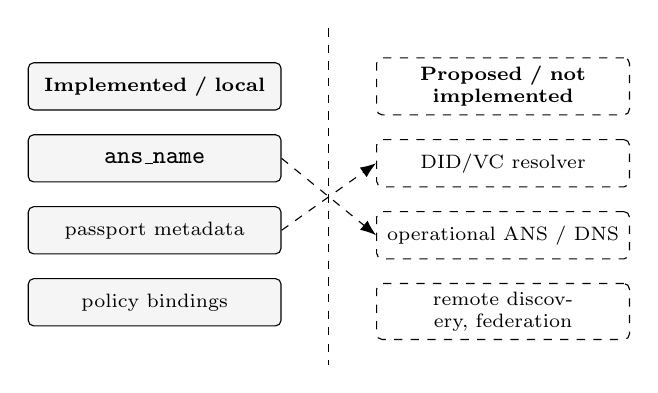
\begin{tikzpicture}[node distance=3mm]
\node[apimpl,text width=30mm] (li) {\textbf{Implemented / local}};
\node[apimpl,below=of li,text width=30mm] (a) {\code{ans\_name}};
\node[apimpl,below=of a,text width=30mm] (b) {passport metadata};
\node[apimpl,below=of b,text width=30mm] (c) {policy bindings};
\node[approp,right=12mm of li,text width=30mm] (ri) {\textbf{Proposed / not implemented}};
\node[approp,below=of ri,text width=30mm] (d) {DID/VC resolver};
\node[approp,below=of d,text width=30mm] (e) {operational ANS / DNS};
\node[approp,below=of e,text width=30mm] (f) {remote discovery, federation};
\draw[apdash] (b.east) -- (d.west);
\draw[apdash] (a.east) -- (e.west);
\begin{scope}[on background layer]
\draw[dashed] ($(li.north east)!0.5!(ri.north west) + (0,4mm)$)
  -- ($(c.south east)!0.5!(f.south west) - (0,4mm)$);
\end{scope}
\end{tikzpicture}
\caption{Boundary between local metadata and external verification. Left items
are implemented as local declarations; right items are proposed and unbuilt;
dashed edges are not-yet-implemented links.}
\label{fig:boundary}
\end{figure}

\section{Background and Motivation}\label{sec:background}

\subsection{Why external metadata is hard to review}
When sovereign metadata lives outside the executable artifact, three failure
modes follow that the passport is designed to address: a reviewer cannot tell an
\emph{omitted} constraint from an \emph{approved} one; two artifacts (e.g., a
manifest and the running program) can silently disagree; and a favorable
human-facing summary can mask an unfavorable underlying decision.

\subsection{Naming vs.\ identity vs.\ credentials vs.\ policy}
A recurring category error conflates four distinct functions. A \emph{resolvable
name} answers ``where is the record?''. An \emph{authenticated identity} answers
``who controls the relevant key or account?''. A \emph{credential} answers a
scoped, issuer-signed assertion. A \emph{policy decision} answers ``is this
operation permitted in context?''. These cannot substitute for one another. The
Agent Passport deliberately occupies only the \emph{local declaration} slice of
this space: it records a local name and locally asserted metadata and binds them
to policy declarations, without claiming to resolve, authenticate, or verify
anything external.

\subsection{Why residency and jurisdiction metadata matter}
Data-residency and jurisdiction constraints are increasingly first-order
governance inputs for agent deployments operating across regions. Today these
constraints are usually informal. Making them \emph{explicit and compile-checked}
---even as declarations---lets a runtime record which residency set and
jurisdiction accompanied an operation, and lets a reviewer detect when a declared
residency value lies outside an allowed set. This is an auditability benefit, not
an enforcement guarantee: a declared residency of \code{EU} does not prove that
bytes were stored in the EU.

\subsection{Distinguishing the passport from adjacent systems}
DID/VC \cite{w3c_did_core_2022,w3c_vc_data_model_2025} define \emph{external}
identity and credential models with cryptographic control and issuer signatures;
the passport stores only local declarations unless a resolver/verifier is
implemented, and none is here. DNS / naming / NANDA-style discovery
\cite{mockapetris1987dnsconcepts,projectnanda2026,raskar2025beyonddns} provide
operational resolution; the passport's \code{ans\_name} is local metadata and
operational discovery is proposed, not implemented. MCP/A2A
\cite{mcp_spec_2025,a2a_spec} standardize interaction; passport metadata can
bind to such boundaries but no live interoperability is implemented here.
Policy-as-code (OPA) \cite{opa_docs} is an external decision engine; \Argorix
compiles policy metadata and passport bindings together with the program.

\section{Agent Passport Model}\label{sec:model}

\subsection{Definition}
An \emph{Agent Passport} is a local, compiled declaration that collects locally
asserted identity and governance context for one subject agent. Its fields are:
a \emph{passport name} (local identifier); a \emph{subject agent} (reference to
an agent declared in the same program); \emph{country} (observed \code{CL});
\emph{jurisdiction} (observed \code{CL}); \emph{permitted residency} (a set of
allowed values, observed \code{CL} and \code{EU}); \emph{capabilities};
\emph{policy bindings} (references to policy declarations); an \code{ans\_name}
(local agent naming field); and optional \emph{identity / credential / trust
metadata} referencing identity, credential, and ATrust declarations
\cite{vazquez_atrust}. The passport relates to agent declarations (the subject),
policies (bindings), runtime profiles (which govern runtime behavior), and
evidence requirements (which determine what is emitted).

\subsection{What the passport is---and is not}
The passport \emph{is} a local compiled declaration that creates a typed,
inspectable, runtime-visible metadata boundary; within the compiled program it
binds a name and sovereign metadata to a specific agent and policies, and that
binding is checked. The passport \emph{is not} a government document, \emph{is
not} legal identity, \emph{does not} verify external identity, and \emph{does
not} prove physical data residency. \emph{Sovereign} here denotes explicit
jurisdictional and residency metadata controlled by the program, not state
recognition or legal status. No external registry validates the declared
country, jurisdiction, or residency values. Table~\ref{tab:fields} summarizes the
fields and their assurance ceiling, and Fig.~\ref{fig:binding} shows the binding
model.

\begin{figure}[t]
\centering
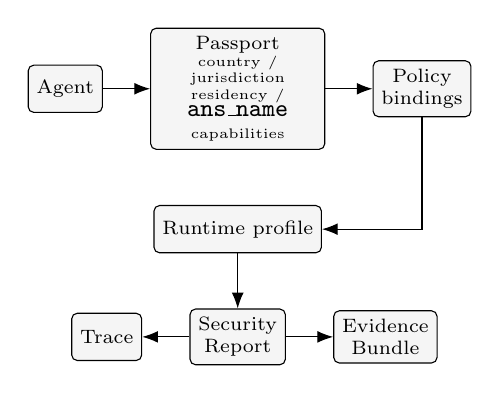
\begin{tikzpicture}[node distance=5mm and 6mm]
% Top row: agent -> passport -> policy bindings
\node[apimpl] (agent) {Agent};
\node[apimpl,right=of agent,text width=20mm] (pass)
  {Passport\\{\tiny country / jurisdiction\\ residency / \code{ans\_name}\\ capabilities}};
\node[apimpl,right=of pass] (pol) {Policy\\bindings};
% Middle: runtime profile centred below the passport
\node[apimpl,below=7mm of pass] (prof) {Runtime profile};
% Bottom row: evidence artifacts
\node[apimpl,below=7mm of prof] (sr) {Security\\Report};
\node[apimpl,left=of sr] (tr) {Trace};
\node[apimpl,right=of sr] (eb) {Evidence\\Bundle};
\draw[apflow] (agent) -- (pass);
\draw[apflow] (pass) -- (pol);
\draw[apflow] (pol.south) |- (prof.east);
\draw[apflow] (prof) -- (sr);
\draw[apflow] (sr) -- (tr);
\draw[apflow] (sr) -- (eb);
\end{tikzpicture}
\caption{Agent Passport binding model. Edges denote validated in-program
references and preserved metadata, not verified real-world relationships.}
\label{fig:binding}
\end{figure}

\begin{table}[t]
\centering
\caption{Agent Passport fields and semantics.}
\label{tab:fields}
\renewcommand{\arraystretch}{1.2}
\footnotesize
\begin{tabular}{@{}p{0.20\columnwidth}p{0.34\columnwidth}p{0.30\columnwidth}@{}}
\toprule
\textbf{Field} & \textbf{Meaning / implemented status} & \textbf{External assurance claim} \\
\midrule
Passport name & Local identifier; parsed, validated, lowered, emitted & None \\
Subject agent & Reference to in-program agent; resolution enforced & None \\
Country & Declared; preserved into evidence (declarative) & None (not validated) \\
Jurisdiction & Declared; preserved into evidence (declarative) & None \\
Permitted residency & Allowed value set; membership-checkable & None (no physical proof) \\
Capabilities & Capability references; binding validated & None beyond local checks \\
Policy bindings & References to policies; resolution enforced & None (binding $\neq$ approval) \\
\code{ans\_name} & Local naming field; survives to artifacts & None (no DNS/DID/registry) \\
Identity/\allowbreak cred./\allowbreak trust & References into declarations; validated & None (no issuance/\allowbreak verify) \\
\bottomrule
\end{tabular}
\end{table}

\section{Compilation and Semantic Validation}\label{sec:compile}
\Argorix groups declarations into modules and processes them through five
relevant stages; passports traverse all five.
\emph{(1) Parsing} produces a source-faithful AST; passport declarations are
retained structurally, not rewritten or discarded.
\emph{(2) Name and module resolution} binds declarations without discarding
provenance, so a passport's subject-agent and policy-binding references resolve
against the program's declared names.
\emph{(3) Semantic analysis} checks uniqueness, references, cross-construct
constraints, and denied combinations: the subject agent must exist; each policy
binding must reference an existing policy; residency values must belong to an
allowed declaration set; identity/credential/trust references must resolve.
\emph{(4) Lowering} converts only validated forms to IR and serializable
bytecode, \emph{preserving} passport metadata rather than erasing it.
\emph{(5) VM execution} loads bytecode, installs only explicitly executable
providers, and evaluates policy before scheduling work, making passport
constraints and metadata available to the evidence pipeline.

This ordering matters: a runtime-only check discovers invalid configuration
after deployment, and an unchecked lowering pass can erase the distinction
between an omitted field and an approved one.

\subsection{Declarative metadata vs.\ executable controls}
\emph{Executable runtime controls} (e.g., the fail-closed provider boundary,
network/secret denial) change what the runtime \emph{does}. \emph{Declarative
metadata} (country, jurisdiction, residency, identity/credential references,
\code{ans\_name}) is validated and preserved but does not, by itself, perform an
external action. The passport is primarily declarative metadata with implemented
binding/validation and implemented evidence preservation; it does not execute
identity verification or residency enforcement.

\subsection{Validation rules}
Let $P$ be a passport, $A$ the declared agents, $\Pi$ the declared policies, and
$R$ the allowed residency declaration set. Table~\ref{tab:rules} states the six
rules, their condition, and the effect when the condition is not met.

\begin{table}[t]
\centering
\caption{Passport semantic validation rules.}
\label{tab:rules}
\renewcommand{\arraystretch}{1.25}
\setlength{\tabcolsep}{4pt}
\footnotesize
\begin{tabular}{@{}p{0.07\columnwidth}p{0.42\columnwidth}p{0.39\columnwidth}@{}}
\toprule
\textbf{Rule} & \textbf{Condition} & \textbf{Effect} \\
\midrule
R1 & \code{P.subject}~$\in A$ & reject: dangling agent reference \\
R2 & \code{b}~$\in \Pi$ for each policy binding & reject: dangling policy reference \\
R3 & \code{r}~$\in R$ for each residency value & reject: residency outside set \\
R4 & \code{ans\_name} is local metadata only & no resolution/\allowbreak authentication (no resolver) \\
R5 & identity/\allowbreak credential/\allowbreak trust refs stay declarative & no verification (no verifier) \\
R6 & emit \code{lower(P)} iff R1\,$\wedge$\,R2\,$\wedge$\,R3 & country/\allowbreak jurisdiction/\allowbreak residency/\allowbreak\code{ans\_name} kept in IR/\allowbreak bytecode \\
\bottomrule
\end{tabular}
\end{table}

Rules R1--R3 are enforced bindings/validations; R4--R5 are \emph{boundary} rules
describing the semantic ceiling of a validated passport; R6 makes explicit that
successful lowering is conditioned on reference and membership validity and that
the surviving metadata is what later appears in evidence. None of these rules
establishes that a declared value is externally \emph{true}.

\section{Runtime Evidence Path}\label{sec:evidence}
Passport metadata becomes auditable because it is carried into runtime evidence
artifacts. Each \emph{complete} request directory contains five artifacts:
source (\code{session.argx}), compiled bytecode (\code{session.argbc.json}), a
trace (\code{session.trace.json}), a security report
(\code{session.security.json}), and an evidence bundle
(\code{session.evidence.json}).

The \emph{trace} is an ordered ledger of compiler/VM and policy events; among its
declaration events, each complete trace records declarations for two agents, six
policies, \emph{two passports}, plus governance, threat, conformance, release,
ATrust, MCP, and A2A metadata. Passport declarations therefore appear in the
runtime ledger, not only in source. The \emph{SecurityReport} is a structured
interpretation of runtime evidence: execution status, policy results, review
state, provider boundary, and declared controls. The \emph{EvidenceBundle}
records four semantic SHA-256 digests---\code{bytecode\_digest},
\code{trace\_digest}, \code{report\_digest}, and \code{ledger\_digest} (the
canonical digest of \code{trace.events})---and an artifact map of
\code{bytecode\_path}, \code{trace\_path}, and \code{security\_report\_path}.
There is no source path or source digest and no standalone ledger path.

Digests are semantic (computed over canonical JSON, independent of whitespace or
key ordering), and \emph{offline verification} recomputes them and the ledger
digest without network access or provider credentials. The detailed verification
algorithm is given in the original preprint \cite{venegas2026argorixlang}; the
point here is its scope: it
begins at compiled bytecode and never asserts that \code{session.argx} produced
it, so passport metadata is verified \emph{as carried into bytecode and trace},
not as traced back to source (Fig.~\ref{fig:evpath}).

\begin{figure*}[t]
\centering
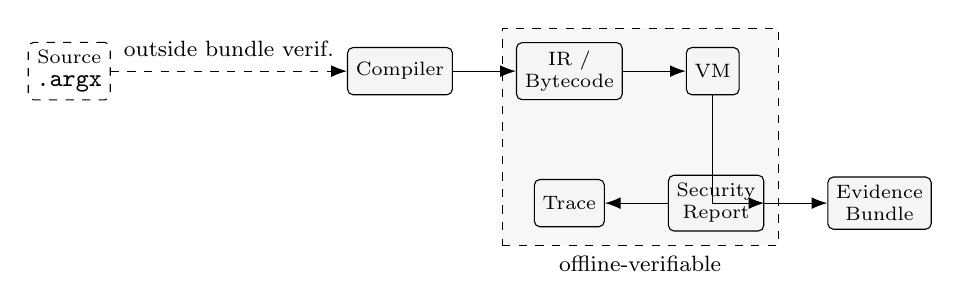
\begin{tikzpicture}[node distance=8mm,every node/.style={font=\footnotesize}]
\node[approp] (src) {Source\\\code{.argx}};
\node[apimpl,right=30mm of src] (cmp) {Compiler};
\node[apimpl,right=of cmp] (bc) {IR /\\Bytecode};
\node[apimpl,right=of bc] (vm) {VM};
\node[apimpl,below=10mm of bc] (tr) {Trace};
\node[apimpl,right=of tr] (sr) {Security\\Report};
\node[apimpl,right=of sr] (eb) {Evidence\\Bundle};
\draw[apdash] (src) -- node[midway,above=0.6mm,font=\footnotesize]{outside bundle verif.} (cmp);
\draw[apflow] (cmp) -- (bc);
\draw[apflow] (bc) -- (vm);
\draw[apflow] (vm.south) |- (sr.east);
\draw[apflow] (sr) -- (tr);
\draw[apflow] (sr) -- (eb);
\begin{scope}[on background layer]
\node[draw,dashed,fill=black!3,fit=(bc)(tr)(sr),inner sep=5pt,label=below:{\footnotesize offline-verifiable}] {};
\end{scope}
\end{tikzpicture}
\caption{Runtime evidence path. The source-to-compiler edge is dashed and lies
outside bundle verification; bytecode, trace, and report form the
offline-verifiable region (semantic digests plus ledger digest).}
\label{fig:evpath}
\end{figure*}

\noindent\textbf{Key claim.} The Agent Passport lets runtime consumers
\emph{inspect which sovereign metadata and policy bindings accompanied an agent
operation}. It does \emph{not} prove the metadata is externally true. Three
orthogonality statements bound this: a valid digest detects content change
relative to the bundle but does not prove who created it; a linked trace does not
prove that events outside the instrumented runtime did not occur; and artifact
integrity does not turn a failing policy result into approval. No signature,
trusted timestamp, transparency service, hardware root, or independent witness is
evaluated here. Bundle integrity therefore does \emph{not} imply legal
compliance, certification, authentication, or policy approval.

\section{Observational Evaluation}\label{sec:eval}
We reuse the existing \Argorix runtime artifact corpus. All values are taken
directly from the source preprint's normalized datasets
\cite{venegas2026argorixlang}; we add no new experiment.

\subsection{Corpus and completeness}
Of \textbf{33} request directories, \textbf{27} (81.8\%) contain all five
expected artifacts and \textbf{6} (18.2\%) contain source only. All 27 complete
sessions report execution status \code{completed}; execution status is
unavailable for the six source-only directories, which cannot be assessed for
trace-level fields. We retain the six as explicit incomplete observations.

\subsection{Offline bundle verification}
All \textbf{27/27} complete bundles pass the repository's offline verifier. For
each, the bytecode, trace, security-report, and trace-event-ledger digest fields
are syntactically valid SHA-256 identifiers, the three semantic digests
reproduce, the ledger digest recomputes from trace events, and the LedgerSummary
digest matches. The verifier does not digest or verify \code{session.argx}.
Verification establishes internal cross-artifact consistency, not producer
authentication, absence of side effects, or policy approval.

\subsection{Passport evidence}
Every complete session reports \textbf{two passports}, with country and
jurisdiction Chile (\code{CL}) and data-residency declarations including
\code{CL} and \code{EU}. These values demonstrate that sovereign metadata
survives compilation and appears in runtime evidence. They do \emph{not} show
that data was physically stored in either region, nor that any external registry
validated the declarations.

\subsection{Prompt-content availability}
The bounded \code{injected.content} field is present in \textbf{0 of 27}
complete, valid traces; the six source-only directories have no trace and are not
assessable. Consequently no qualitative prompt themes, quotations, injection
labels, or attack-success rates can be reported---simultaneously a
data-minimization benefit and an evaluation limitation. Table~\ref{tab:obs}
summarizes the observed passport evidence.

\begin{table}[t]
\centering
\caption{Observed passport evidence in the runtime corpus.}
\label{tab:obs}
\renewcommand{\arraystretch}{1.2}
\footnotesize
\begin{tabular}{@{}p{0.40\columnwidth}p{0.16\columnwidth}p{0.30\columnwidth}@{}}
\toprule
\textbf{Measure} & \textbf{Observed} & \textbf{Interpretation} \\
\midrule
Request directories & 33 & Full corpus \\
Complete sessions (5 artifacts) & 27 & Assessable for trace fields \\
Source-only sessions & 6 & Not assessable \\
Bundles passing offline verification & 27 / 27 & Internal consistency only \\
Passports per complete session & 2 & Metadata survives to evidence \\
Country / jurisdiction & \code{CL} / \code{CL} & Declaration, not validated \\
Residency declarations & \code{CL}, \code{EU} & Not physical-residency proof \\
Traces with \code{injected.content} & 0 / 27 & No prompt-level analysis \\
\bottomrule
\end{tabular}
\end{table}

\subsection{Interpretation}
The corpus demonstrates that passport metadata can be compiled and preserved into
runtime evidence and that complete bundles are offline-consistent. It does
\emph{not} demonstrate real identity authentication, DID/VC verification,
operational DNS/ANS resolution, legal compliance, or physical residency
enforcement. The repeated structure across complete sessions supports pipeline
reproducibility but weakens any claim about behavioral diversity.

\section{Security and Governance Analysis}\label{sec:security}
We analyze threats as attack paths across trust boundaries, not as proof that a
named control defeats every adversary.

\noindent\textbf{Threats.} \emph{Identity spoofing}: a program may declare
arbitrary identity/credential references; local checks prevent dangling
references but cannot establish that a referenced identity is genuine.
\emph{False residency declaration}: \code{permitted\_residency} may be any in-set
value; membership is checked but truthfulness is not. \emph{Policy confusion}: a
consumer reading only a coarse top-level status could overlook an unfavorable
detailed result. \emph{Metadata laundering}: re-emitting a self-consistent bundle
with attacker-chosen sovereign metadata is possible if the bundle is unsigned and
artifacts and bundle are replaced together. \emph{Overreading}: the most
pervasive risk is treating a local declaration as external assurance.

\noindent\textbf{Bounded mitigations.} Semantic validation rejects dangling
references and out-of-set residency values (R1--R3, R6); explicit claim
boundaries (Table~\ref{tab:claim}) keep declarative metadata from being promoted
to assurance; evidence linkage via semantic digests detects content change
relative to a bundle; review states preserve component-level policy status; and
separation of local naming from operational discovery prevents a validated
\code{ans\_name} from being mistaken for a resolved identity.

\noindent\textbf{Remaining risks.} Malicious-but-well-formed declarations, fake
credentials, resolver attacks (once a resolver exists), missing revocation,
adapter compromise, and unsigned bundles all remain in scope for future testing.
The strongest supported statement is conditional: within the observed runtime
path, requests are mediated by compiled policy and an executable-provider
allowlist, denials are recorded, passport metadata is preserved, and complete
artifacts are offline-consistent. Security outside that path is unmeasured.
Table~\ref{tab:threats} states the bounded mitigation claims.

\begin{table}[t]
\centering
\caption{Threats and bounded mitigations (passport-focused).}
\label{tab:threats}
\renewcommand{\arraystretch}{1.2}
\footnotesize
\begin{tabular}{@{}p{0.34\columnwidth}p{0.34\columnwidth}p{0.20\columnwidth}@{}}
\toprule
\textbf{Threat} & \textbf{Bounded mitigation} & \textbf{Claim status} \\
\midrule
Dangling identity/policy ref & Semantic reference validation & Implemented \\
Residency outside allowed set & Membership check (R3) & Implemented \\
Policy confusion (coarse vs.\ detailed) & Preserved component status / review & Implemented \\
Evidence tampering & Digest-linked bundle & Implemented (no producer auth) \\
False/unverified external identity & --- (verifier not implemented) & Not claimed \\
Physical residency enforcement & --- & Not claimed \\
\bottomrule
\end{tabular}
\end{table}

\section{Related Work}\label{sec:related}
We compare carefully and claim no equivalence. DID Core and Verifiable
Credentials \cite{w3c_did_core_2022,w3c_vc_data_model_2025} provide external
identity and credential models with cryptographic control and issuer signatures;
the passport stores only local declarations and validated references and performs
no DID resolution or credential verification unless a verifier is added. DNS /
naming / NANDA-style discovery
\cite{mockapetris1987dnsconcepts,mockapetris1987dnsimplementation,projectnanda2026,raskar2025beyonddns}
provide operational resolution and verified agent facts; the passport's
\code{ans\_name} is local metadata, and sovereign DNS/ANS discovery is proposed
future work. MCP and A2A \cite{mcp_spec_2025,a2a_spec} standardize interaction
surfaces; passport metadata can bind to MCP/A2A boundary declarations, but no
live interoperability is implemented. OPA \cite{opa_docs} decouples policy
decision from enforcement as an external engine; \Argorix instead compiles
policy metadata and passport bindings within the program. in-toto
\cite{torresarias2019intoto} provides signed supply-chain guarantees; \Argorix
EvidenceBundles are local, unsigned, semantic-digest bundles unless extended.
WASI \cite{wasi_intro} provides host-level capability isolation; the passport
model makes no host-isolation claim. Agent languages
\cite{bordini2007jason} and AI-risk and LLM-security guidance
\cite{tabassi2023airmf,owasp_llm_top10} provide complementary framing.

\begin{table*}[t]
\centering
\caption{Claim-boundary taxonomy (sovereign-metadata view).}
\label{tab:claim}
\renewcommand{\arraystretch}{1.25}
\footnotesize
\begin{tabular}{@{}p{0.13\textwidth}p{0.20\textwidth}p{0.18\textwidth}p{0.17\textwidth}p{0.19\textwidth}@{}}
\toprule
\textbf{Concept} & \textbf{Implemented} & \textbf{Declarative} & \textbf{Proposed} & \textbf{Not claimed} \\
\midrule
Local naming & \code{ans\_name} binding, preserved & sovereign naming metadata & operational ANS/DNS & DNS/registry resolution \\
Identity / cred. & reference validation & identity/cred.\ refs, ATrust maps & DID/VC resolver, signed attest. & external auth, cred.\ verify \\
Jurisdiction / residency & evidence preservation; membership check & country/juris./residency decls & --- & legal cert., physical proof \\
Policy binding & reference resolution; profile binding & policy associations & decision canonicalization & binding-as-approval \\
Evidence & semantic-digest bundle, offline verify & trace/report fields & signed bundles, transparency log & producer auth, immutability \\
Provider boundary & fail-closed path, simulated allowlist & contract metadata & live federation & external exec, prod.\ isolation \\
\bottomrule
\end{tabular}
\end{table*}

\section{Limitations}\label{sec:limits}
We state limitations strictly. There is \emph{no} external identity verification;
\emph{no} DID/VC resolver; \emph{no} cryptographic proof of control (no
handshake, challenge--response, or key-control proof); \emph{no} legal-compliance
certification of declared country/jurisdiction/residency; \emph{no} physical
residency enforcement; \emph{no} production-isolation proof (runtime denials are
VM-level control-flow properties, with OS/process/network/secret-store
containment untested); \emph{no} controlled adversarial experiment (the corpus
has no prompt text and no controlled attacks, so no injection success rate is
reported); and \emph{no} live provider federation (only a \code{simulated}
provider is executable; external execution is recorded as blocked). Source
integrity is outside bundle verification, and bundles are unsigned. Complete
sessions are structurally uniform, limiting generalization across prompts,
jurisdictions, and policy sets.

\section{Future Work}\label{sec:future}
DID/VC resolver integration to turn declarative identity/credential references
into verifiable claims (introducing trust anchors, replay, revocation, privacy,
and network-failure concerns); signed passport attestations and signed
EvidenceBundles for producer authentication and non-repudiation; source-digest
inclusion so verification extends to \code{session.argx}; a transparency log for
independent witnessing; an operational ANS / Sovereign DNS prototype giving
\code{ans\_name} real resolution semantics; policy-decision canonicalization into
one tri-state decision from typed component results; controlled adversarial
evaluation once prompt content is available under an allowlist; host-level
sandbox measurements; and cross-provider runtime tests with live adapters.

\section{Conclusion}\label{sec:conclusion}
The Agent Passport provides a compiled, evidence-visible metadata boundary for
governed AI agents. It represents sovereign metadata---country, jurisdiction,
permitted residency, capabilities, policy bindings, and a local
\code{ans\_name}---as a typed, semantically validated declaration; lowers
validated metadata into IR and bytecode; and preserves it into traces, security
reports, and offline-verifiable evidence bundles. An observational study of an
existing corpus shows that passport metadata survives compilation and appears in
27/27 complete, offline-consistent sessions, each carrying two passports with
declared Chilean country/jurisdiction and \code{CL}/\code{EU} residency. The
construct's value is not external truth. It is explicit representation, semantic
validation, runtime visibility, and claim-bounded auditability: a runtime
consumer can inspect which sovereign metadata and policy bindings accompanied an
operation, while the metadata remains a local declaration rather than verified
identity, certified compliance, or physical-residency proof.

\section{Scope}\label{sec:diff}
This paper extends and narrows the \Argorix preprint
\cite{venegas2026argorixlang} by focusing specifically on the Agent Passport
construct and its sovereign-metadata evidence path. The ATrust and DCP-AI
conceptual framing \cite{vazquez_atrust,naranjo_dcpai} and the full
language/runtime are treated there; here all empirical values are reused
unchanged, and no new experiment, benchmark, deployment, or security guarantee is
introduced.

\bibliographystyle{IEEEtran}
\bibliography{references}

\end{document}
